\section{Loopshaping}
The first attempt to control the positioning of the cart consists in the simplest technique of directly shaping the bode diagram of the open loop tranfer function. 

\begin{figure}[H]
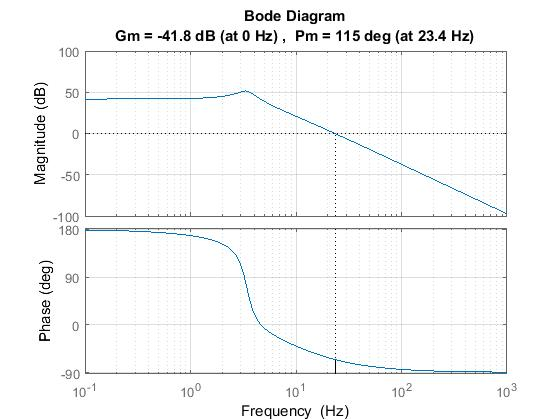
\includegraphics[width=0.5\textwidth]{img/ls_bode_ol.jpg}
\caption{Bode diagram of the loop transfer function of the plant (motor and cart).}
\end{figure}

We consider the simplest model in order to perform the tuning of the controller. The motor and cart are represented by the linear tranfer functions 
\begin{equation}
F(s) = \frac{K_e}{Ls+R} \qquad X(s) = \frac{1}{Ms^2+Cs+K}
\end{equation}
connected in series, where $F(s)$ represents the linear force exerted by the motor and $X(s)$ the position of the cart. The parameters have been identified as explained in detail in the previous section. It is important to remind that the identification has been performed without scaling the encoder values into centimeters; this means that the conversion tofro centimeters must be performed outside the control loop.\\

The openloop plant described by the equations above has three poles: one high frequency pole coming from the motor dynamic, and two complex conjugate poles placed nearby the imaginary axis. The latters are responsible from the oscillatory behaviour of the cart and need to be canceled out from the openloop. Furthermore, the dynamic does not contain any integral action, so we need to introduce it in the controller if we want to achieve zero static error at regime (namely, a perfect positioning of the cart).\\

The considered model for the controller is then:
\begin{equation}
R(s) = K_R\frac{(s+z)(s+z^*)}{s(s+100)}
\end{equation}
where $z,z^*$ are the openloop complex conjugate poles of the plant, which are trivially dependant on the configuration of the plant (namely, spring and mass). Since we do not know the exact position of this pair of poles (making it impossible to perfectly cancel them out), it is better to position the pair of zeros on the left side of the expected position; in this way we are attracting the poles away from the imaginary axis. The pole in $s=-100$ is only needed to obtain a causal regulator and its positioning in high frequency will not perturb the control dynamic in any way. Eventually, the controller gain has to be tuned in order to obtain a desired cutoff frequency which will affect the response time of the controlled plant as well as its stability. \\

\begin{figure}
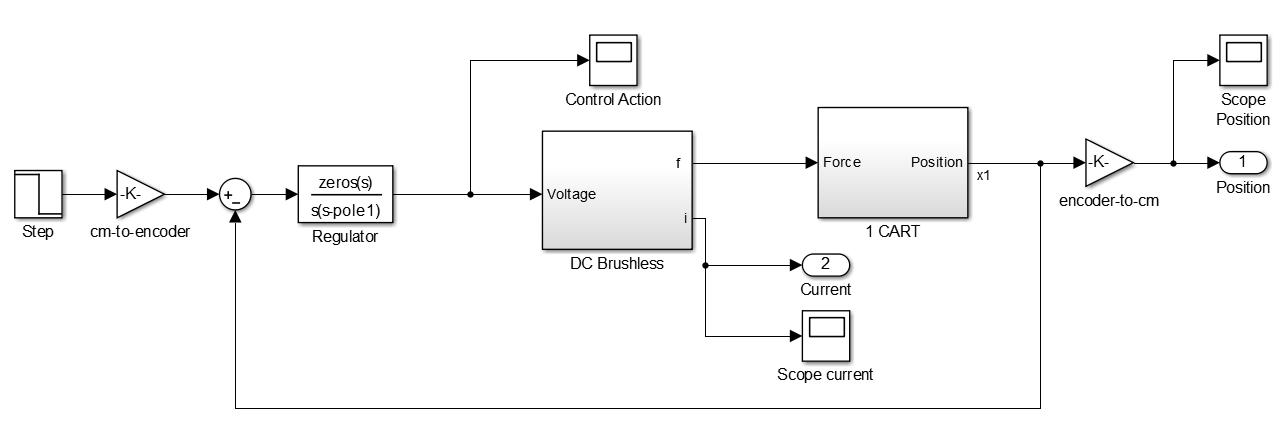
\includegraphics[width=\textwidth]{img/ls_simulink.png}
\caption{Simulink model used for verification of the control design.}
\end{figure}

We then build a simulink model to fine tune the parameters taking into account the saturation of the control input, which affects the maximum bandwidth achievable. The challenge is to push the performances (bandwidth) as close as possible to the saturation of the actuator: this way we are getting the best performance allowed in the linear region of operability. The target output we expect is a positioning time below one second, resulting in a bandwidth around 1 Hz.\\

\begin{figure}[H]
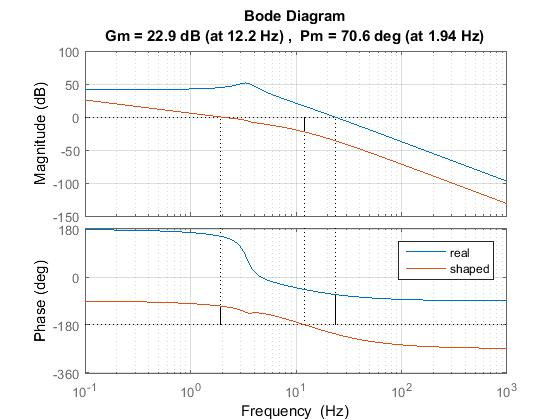
\includegraphics[width=0.5\textwidth]{img/ls_bode_shaping.jpg}
\caption{Bode diagram of the loop transfer function after the shaping.}
\end{figure}

Once satisfied with the simulation, it is time to upload the controller onto Arduino for the real test. We cannot expect that the output of the simulink model will perfectly match the real test, but we do expect to see the same settling time, gain and no saturation for the actuator. As expected the transient does not match the simulink model (which is probably due to the not considered nonlinearities of the plant), but this difference can hardly be detected by the naked eye. 

\begin{figure}[H]
\begin{subfigure}{0.49\textwidth}
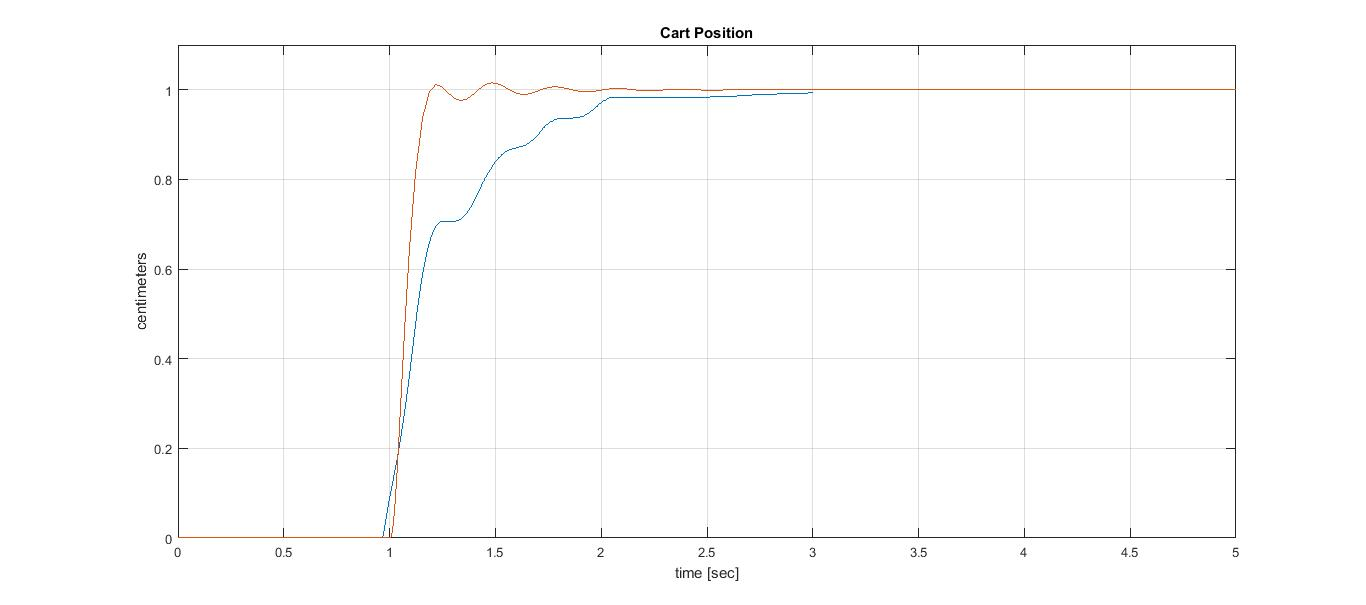
\includegraphics[width=\textwidth]{img/ls_response_kh.jpg}
\caption{Strongest spring.}
\end{subfigure}

\begin{subfigure}{0.49\textwidth}
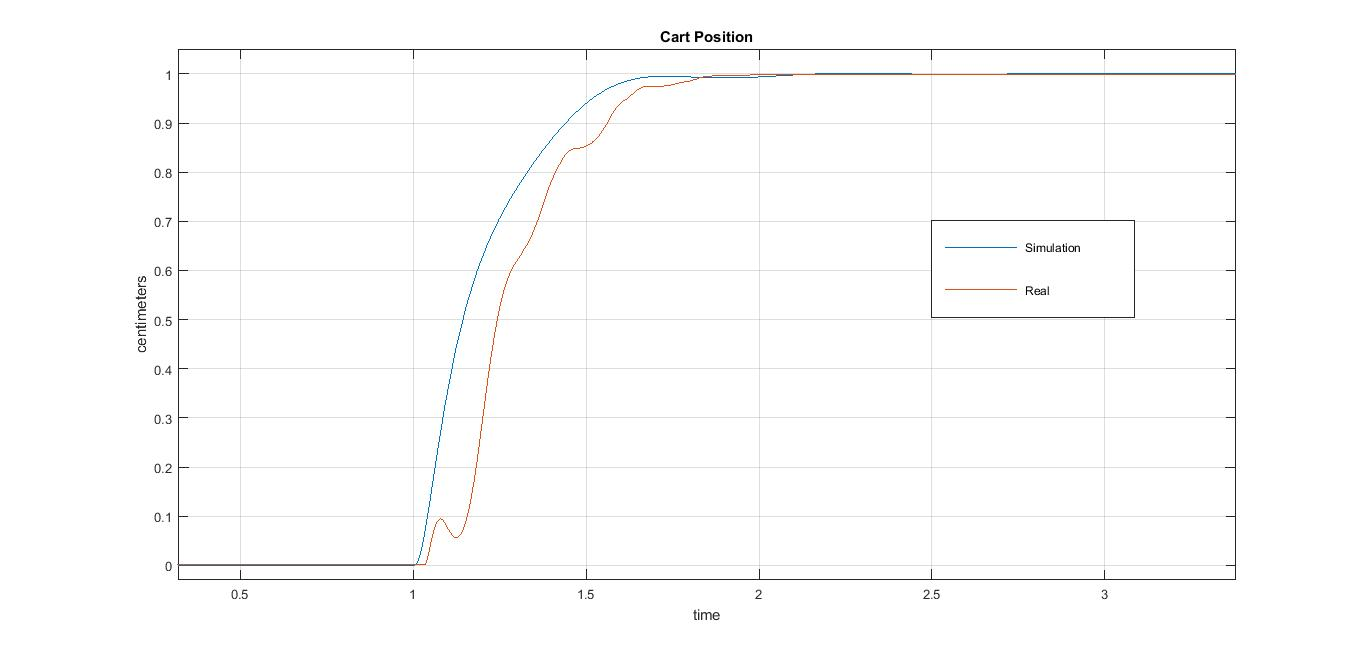
\includegraphics[width=\textwidth]{img/ls_response_kl.jpg}
\caption{Weakest Spring.}
\end{subfigure}

\caption{Comparisons of the step response between the simulated system and the real one.}
\end{figure}
